\documentclass[sigconf,10pt,review,anonymous]{acmart}\settopmatter{printfolios=true,printccs=false,printacmref=false}
\renewcommand\footnotetextcopyrightpermission[1]{} 




\usepackage{amssymb}

\usepackage{booktabs}  
\usepackage{subcaption}
\usepackage[normalem]{ulem}
\usepackage{amsmath}
\usepackage{pifont}
\usepackage{xfrac}
\usepackage{algorithm}
\usepackage{algpseudocode}
\usepackage{url}
\usepackage{comment}
\usepackage{color}
\usepackage{fancyvrb}
\usepackage{balance}
\usepackage{listings}
\usepackage{multirow}
\usepackage{enumitem}
\usepackage{mathtools}
\usepackage{graphicx}
\usepackage{pbox}
\usepackage{makecell}
\usepackage{rotating}
\usepackage{adjustbox}
\usepackage{amsthm}
\usepackage{mathtools}
\usepackage{hyperref}

\usepackage[compatibility=false,font=small,labelfont=bf]{caption}
\lstset{ 
aboveskip=5pt,
belowskip=0pt,
lineskip= 0pt,
language=C++,                % the language of the code
basicstyle=\scriptsize,       % the size of the fonts that are used for the code
numbers=left,                   % where to put the line-numbers
numberstyle=\scriptsize,      % the size of the fonts that are used for the line-numbers
stepnumber=1,                   % the step between two line-numbers. If it's 1, each line 
                                % will be numbered
numbersep=2pt,                  % how far the line-numbers are from the code
backgroundcolor=\color{white},  % choose the background color. You must add \usepackage{color}
showspaces=false,               % show spaces adding particular underscores
stringstyle=\scriptsize,
identifierstyle=\scriptsize,
commentstyle=\scriptsize,
basicstyle=\scriptsize\ttfamily,
%stringstyle=\ttfamily,
showstringspaces=false,         % underline spaces within strings
showtabs=false,                 % show tabs within strings adding particular underscores
frame=t,                   % adds a frame around the code
%framexleftmargin=2mm,
tabsize=2,                      % sets default tabsize to 2 spaces
captionpos=b,                   % sets the caption-position to bottom
floatplacement=t,
breaklines=true,                % sets automatic line breaking
breakatwhitespace=false,        % sets if automatic breaks should only happen at whitespace
title=\lstname,                 % show the filename of files included with \lstinputlisting;
                                % also try caption instead of title
keywordstyle=\color{red}\underbar,                                
escapechar={@},
%escapeinside={\%*}{*)},         % if you want to add a comment within your code
morekeywords={}            % if you want to add more keywords to the set
}



% Copyright
%\setcopyright{none}
\setcopyright{acmcopyright}
%\setcopyright{acmlicensed}
%\setcopyright{rightsretained}
%\setcopyright{usgov}
%\setcopyright{usgovmixed}
%\setcopyright{cagov}
%\setcopyright{cagovmixed}


% DOI
\acmDOI{10.475/123_4}

% ISBN
\acmISBN{123-4567-24-567/08/06}

%Conference
\acmConference[WOODSTOCK'97]{ACM Woodstock conference}{July 1997}{El
  Paso, Texas USA}
\acmYear{1997}
\copyrightyear{2016}


\acmArticle{4}
\acmPrice{15.00}

% These commands are optional
%\acmBooktitle{Transactions of the ACM Woodstock conference}

\settopmatter{printacmref=false}

\newcommand{\tool}[0]{\mbox{\textsc{DJXPerf}}}

\begin{document}
\title{Measuring and Optimizing Data Locality in Java}

\begin{comment}
\author{For Double Blind Review}

\affiliation{%
  \institution{Department of Computer Science}
  \institution{College of William and Mary}
  \city{Williamsburg}
  \state{Virginia}
  \postcode{23188}
}
\email{bli11@email.wm.edu}
\end{comment}



\begin{abstract}
This document provides the supplementary materials for the PPoPP 2020 submission. First, it shows the overall overhead analysis. Then this document shows the accuracy analysis, which the existing issues reported by prior work~\cite{Reusable} (four DaCapo 2006 benchamrks~\cite{dacapo} luindex, bloat, lusearch, xalan and SPECJbb2000~\cite{specjbb2000}), are also detected by \tool{}. Finally, this document describes the optimizations under the guidance of \tool{} for Cache2k 1.2.0 \cite{cache2k}, Apache SAMOA \cite{SAMOA}, Apache Commons Collections \cite{Commons} and Java Grande Benchmark JGFMolDynBench \cite{grande} in the Table 1 of the submitted paper.
\end{abstract}

\maketitle

\section{Overall Overhead Analysis}
In figure~\ref{overhead_plot_overall}, we run \tool{} with Renaissance benchmark suite~\cite{Prokopec:2019:RBS:3314221.3314637}, Dacapo2006~\cite{dacapo}, Dacapo 9.12~\cite{dacapo-9.12}, and SPECjvm2008~\cite{specjvm2008} with 5M sampling period. The figure~\ref{overhead_plot_overall} shows that \tool{} typically incurs 5\% runtime and 5\% memory overhead. 

\begin{figure*}
\centering
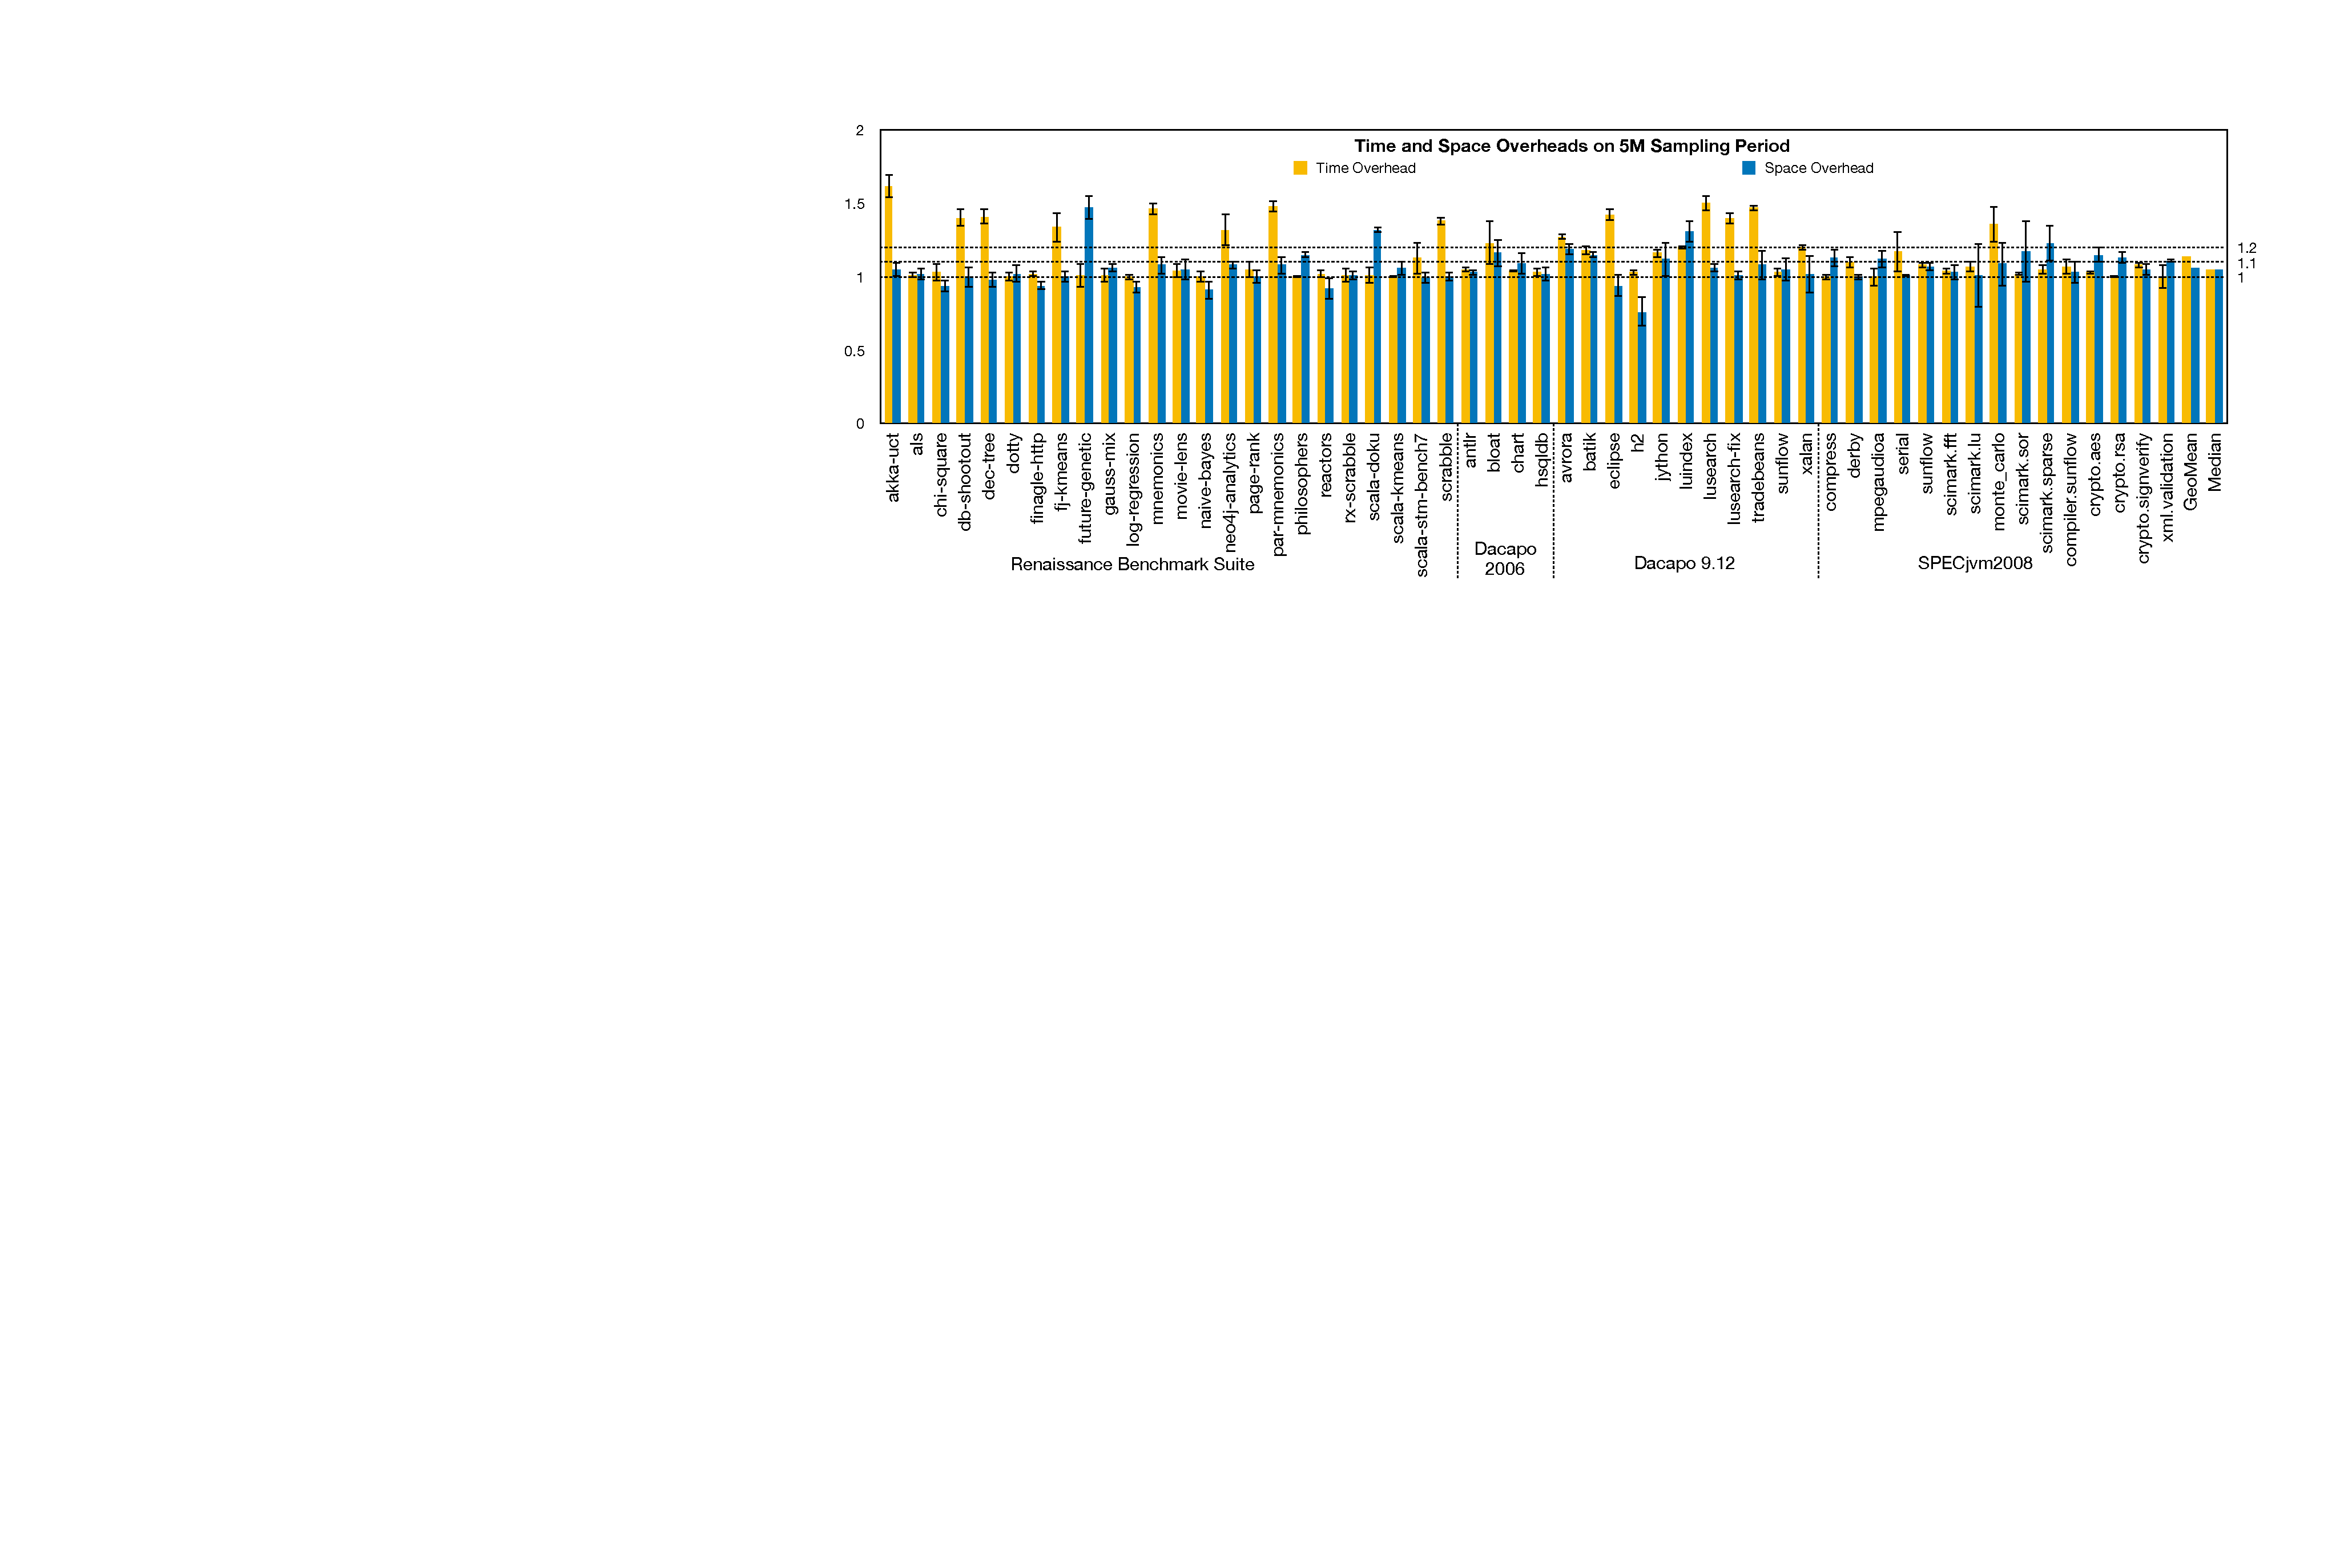
\includegraphics[width=.8\textwidth]{images/overhead_plot_overall.pdf}
\caption{\tool{}'s overall runtime and memory overheads in the unit of times ($\times$) on various benchmarks.}
\label{overhead_plot_overall}
\end{figure*}

\section{Accuracy Analysis}
\subsection{DaCapo 2006 luindex}
luindex uses lucene to indexes a set of documents: the works of Shakespeare and the King James Bible~\cite{dacapo}. \tool{} reports a problematic object---the {\tt Posting} array---allocated at line 235 in method {\tt sortPostingTable} of class {\tt DocumentW-\\riter} reported by prior work~\cite{Reusable}, shown in Listing~\ref{luindex}, which accounts for 23.3\% of total cache misses. We followed the proposed optimizations to fix this issue.

\begin{figure}
\begin{lstlisting}[firstnumber=234,language=java]
private final Posting[] sortPostingTable() {
  @$\blacktriangleright$@Posting[] array = new Posting[postingTable.size()];
  ...
  quickSort(array, ...);
  return array;
}
\end{lstlisting}
\vspace{-0.3in}
\captionof{lstlisting}{DaCapo 2006 luindex: The hotspot object array (line 235) which suffers from memory bloat problem.}
\label{luindex}
\end{figure}

\subsection{DaCapo 2006 bloat}
bloat performs a number of optimizations and analysis on Java bytecode files~\cite{dacapo}. \tool{} reports two problematic objects allocated at line 86 and 91 in the constructor of class {\tt SSAConstructionInfo}: the {\tt LinkedList} object {\tt reals} and the {\tt PhiStmt} object {\tt phis}, shown in Listing~\ref{bloat}. Prior work~\cite{Reusable} did not give the exact source code location they fixed and only mentioned that the issues came from the pervasive created objects in visitor pattern. \tool{} detected such visitor pattern in Figure~\ref{bloat call path}. By checking the calling context in Figure~\ref{bloat call path}, we found that the bloat visits a graph iteratively by creating many visitor objects in nested loops. At the end of the calling context, the program gets into the two problematic objects,  the {\tt LinkedList} object {\tt reals} and the {\tt PhiStmt} object {\tt phis}, which accounts for 13.6\% of total cache misses. To address the problem, we created these two objects outside the constructor {\tt SSAConstructionInfo}. This optimization yields a $(1.07\pm0.02)\times$ speedup.

\begin{figure}
\begin{minipage}{\linewidth}
\scriptsize
 \begin{Verbatim}[commandchars=\\\{\}]
-------------------------------------------------------------
...
EDU.purdue.cs.bloat.cfg.FlowGraph.visit(FlowGraph.java:2249)
EDU.purdue.cs.bloat.tree.TreeVisitor.visitFlowGraph(TreeVisitor.java:94)
EDU.purdue.cs.bloat.cfg.FlowGraph.visitChildren(FlowGraph.java:2235)
EDU.purdue.cs.bloat.cfg.Block.visit(Block.java:167)
EDU.purdue.cs.bloat.tree.TreeVisitor.visitBlock(TreeVisitor.java:99)
EDU.purdue.cs.bloat.cfg.Block.visitChildren(Block.java:162)
EDU.purdue.cs.bloat.tree.Tree.visit(Tree.java:3243)
EDU.purdue.cs.bloat.ssa.SSA.visitTree(SSA.java:110)
EDU.purdue.cs.bloat.tree.IfZeroStmt.visit(IfZeroStmt.java:78)
EDU.purdue.cs.bloat.tree.TreeVisitor.visitIfZeroStmt(TreeVisitor.java:124)
EDU.purdue.cs.bloat.tree.TreeVisitor.visitIfStmt(TreeVisitor.java:114)
EDU.purdue.cs.bloat.tree.TreeVisitor.visitStmt(TreeVisitor.java:219)
EDU.purdue.cs.bloat.tree.TreeVisitor.visitNode(TreeVisitor.java:369)
EDU.purdue.cs.bloat.tree.Node.visitChildren(Node.java:111)
...
\textcolor{red}{EDU.purdue.cs.bloat.ssa.SSAConstructionInfo(SSAConstructionInfo.java:86)}
\textcolor{red}{EDU.purdue.cs.bloat.ssa.SSAConstructionInfo(SSAConstructionInfo.java:91)}
-------------------------------------------------------------
\end{Verbatim}
\end{minipage}
\vspace{-3ex}
\caption{DaCapo 2006 bloat: The hotspot call path to the allocation site line 86 and 91 in SSAConstructionInfo.java.}
\label{bloat call path}
\end{figure}

\begin{figure}
\begin{lstlisting}[firstnumber=84,language=java]
public SSAConstructionInfo(FlowGraph cfg, VarExpr expr) {
  ...
  @$\blacktriangleright$@reals = new LinkedList[cfg.size()];
  allReals = new LinkedList();
  
  defBlocks = new HashSet();
  
  @$\blacktriangleright$@phis = new PhiStmt[cfg.size()];
}
\end{lstlisting}
\vspace{-0.3in}
\captionof{lstlisting}{DaCapo 2006 bloat: The hotspot object reals and phis (line 86 and 91) which suffer from memory bloat problem.}
\label{bloat}
\end{figure}

\subsection{DaCapo 2006 lusearch}
lusearch uses lucene to do a text search of keywords over a corpus of data comprising the works of Shakespeare and the King James Bible~\cite{dacapo}. \tool{} reports a problematic object---the {\tt QueryParser} object---allocated at line 119 in method {\tt parse} of class {\tt QueryParser} reported by prior work~\cite{Reusable}, shown in Listing~\ref{lusearch}, which accounts for 9.2\% of total cache misses. To address the problem, we pulled this allocation site out of the method {\tt parse}. We followed the proposed optimizations to fix this issue.

\begin{figure}
\begin{lstlisting}[firstnumber=118,language=java]
static public Query parse(String query, String field, Analyzer analyzer) {
  @$\blacktriangleright$@QueryParser parser = new QueryParser(field,analyzer);
  return parser.parse(query);
}
\end{lstlisting}
\vspace{-0.3in}
\captionof{lstlisting}{DaCapo 2006 lusearch: The hotspot object parser (line 119) which suffers from memory bloat problem.}
\label{lusearch}
\end{figure}

\subsection{DaCapo 2006 xalan}
xalan transforms XML documents into HTML~\cite{dacapo}. \tool{} reports a problematic object---the {\tt Transformer} object---allocated at line 100 in method {\tt run} of class {\tt XSLTBench} reported by prior work~\cite{Reusable}, shown in Listing~\ref{xalan}, which accounts for 16.7\% of total cache misses. We followed the proposed optimizations to fix this issue.

\begin{figure}
\begin{lstlisting}[firstnumber=96,language=java]
public void run() {
  ...
  while (true) {
    ...
    @$\blacktriangleright$@Transformer transformer=_template.newTransformer();
    ...
  }
  ...
}
\end{lstlisting}
\vspace{-0.3in}
\captionof{lstlisting}{DaCapo 2006 xalan: The hotspot object transformer (line 100) which suffers from memory bloat problem.}
\label{xalan}
\end{figure}

\subsection{SPECJbb2000}
SPECjbb2000 is SPEC's first benchmark for evaluating the performance of server-side Java~\cite{specjbb2000}. \tool{} reports a problematic object---the {\tt Hashtable} object---allocated at line 173 in method {\tt process} of class {\tt StockLevelTransaction} as shown in Listing~\ref{specjbbb2000}, which accounts for 4.7\% of total cache misses. To address the problem, we pulled this allocation site out of the method {\tt process}. This optimization increases the overall throughput by $(1.02\pm0.01)\times$ and no running time speedup.

\begin{figure}
\begin{lstlisting}[firstnumber=171,language=java]
boolean process() {
  ...
  @$\blacktriangleright$@Hashtable stockList = new Hashtable(200);
  ...
}
\end{lstlisting}
\vspace{-0.3in}
\captionof{lstlisting}{SPECJbb2000: The hotspot object stockList (line 173) which suffers from memory bloat problem.}
\label{specjbbb2000}
\end{figure}


\section{Case Studies}
\subsection{Locality Issues due to Memory Bloat}
\subsubsection{Cache2k 1.2.0}
Cache2k~\cite{cache2k} provides an in-memory object cache implementation for Java applications. 
We run Cache2k with provided Cache2k JMH benchmarks as input.
\tool{} reports a problematic object allocated at line 313 in method {\tt rehash} of class {tt Hash2} as shown in Listing~\ref{cache2k}. This object---an array of {\tt Entry} objects that contains key value pairs---accounts for 85.6\% of  total cache misses. 
Further investigation shows that the code repeatedly creates {\tt Entry} object to rehash the entries. Because the Entry object never escapes to the heap, each thread needs only one instance of this data structure at any point during the execution. To address the problem, we create a static {\tt Entry} array that maintains one Entry object per thread. Also, each time an {\tt Entry} object is needed, we will reset this {\tt Entry} array. This optimization yields a $(1.09\pm0.02)\times$ speedup. 


\begin{figure}[h]
\begin{lstlisting}[firstnumber=310,language=java]
private void rehash() {
  Entry<K,V>[] src = entries;
  int i, sl = src.length, n = sl * 2, _mask = n - 1, idx;
  @$\blacktriangleright$@Entry<K,V>[] tab = new Entry[n];
  ...
  entries = tab;
  calcMaxFill();
}
\end{lstlisting}
\vspace{-0.3in}
\captionof{lstlisting}{cache2k: The hotspot object tab (line 313) which suffers from memory bloat problem.}
\label{cache2k}
\end{figure}


\subsubsection{Apache SAMOA}
Apache SAMOA~\cite{SAMOA} (Scalable Advanced Massive Online Analysis) is a platform for mining big data streams. We run Apache SAMOA with the {\tt covtypeNorm.\\arff} dataset as its input. \tool{} reports a problematic object---{\tt Instance}---allocated at line 165 in method {\tt readIns-\\tanceDense} of class {\tt ArffLoader}. This object accounts for 26\% of total cache misses. With code investigation as shown in Listing~\ref{SAMOA}, we find that this {\tt Instance} object is repeatedly formed (line 165) every time the program reads a dense instance from a file, and different instances of this object do not overlap in their life intervals. Thus, we hoist this object outside of the loop and put it into a static location to avoid repeated allocation and. This optimization yields a $(1.17\pm0.04)\times$ speedup to the entire program execution.

\begin{figure}
\begin{lstlisting}[firstnumber=163,language=java]
public Instance readInstanceDense() {
  ...
  @$\blacktriangleright$@Instance instance = newDenseInstance(this.instanceInformation.numAttributes());
  int numAttribute = 0;
  instance.setValue(numAttribute, streamTokenizer.nval);
  ...
}
\end{lstlisting}
\vspace{-0.3in}
\captionof{lstlisting}{Apache SAMOA: The hotspot object instance (line 165) which suffers from memory bloat problem.}
\label{SAMOA}
\end{figure}


\subsubsection{Apache Commons Collections}
Apache Commons Collections~\cite{Commons} include many powerful data structures that accelerate development of most significant Java applications. We run it using its provided commons collections4 map tests as input.
 \tool{} reports a problematic object---the {\tt HashEntry} array---in the constructor of class {\tt AbstractHash-\\edMap}, which is used as a map to store key-value entries. Line 5 of listing~\ref{Commons} shows this object allocation, which accounts for 22\% of total cache misses. 
Similar to other cases that different instances of this object have disjoint life intervals, so we change this object as a static one. When to use a new HashEntry object, we clear and reuse the static object to avoid repeated allocation upon each iteration. The optimization yields a $(1.08\pm0.01)\times$ speedup to the entire program. %The peak memory consumption was reduced from 798684KB to 773704KB (3.1\%).

\begin{figure}
\begin{lstlisting}[firstnumber=1,language=java]
protected AbstractHashedMap(int initialCapacity, final float loadFactor) {
  ...
  this.loadFactor = loadFactor;
  this.threshold = calculateThreshold(initialCapacity, loadFactor);
  @$\blacktriangleright$@this.data = new HashEntry[initialCapacity];
  ...
}
\end{lstlisting}
\vspace{-0.3in}
\captionof{lstlisting}{Apache Commons Collections: The hotspot object data (line 5) which suffers from memory bloat problem.}
\label{Commons}
\end{figure}


\subsection{Issues due to Traditional Locality}
\subsubsection{Java Grande: JGFMolDynBench}

JGFMolDynBench is simple N-body code modeling the behavior of N argon atoms interacting under a Lennard-Jones potential in a cubic spatial volume with periodic boundary conditions~\cite{grande}.
We run JGFMolDynBench with input size B. \tool{} reports the array {\tt md.one} accounts for 83.8\% of the total cache misses and the problematic accesses to this array are highlighted in the method {\tt force} of the class {\tt md}, as shown at line 4, 5, and 6 of Listing~\ref{JGFMolDynBench}. 
The method {\tt force} is called multiple times in a loop (not shown). The loop in method force (line 3) has a streaming access pattern on array {\tt md.one}, which shows up as poor temporal locality. Like JGFMonteCarloBench, we apply loop tiling to improve the temporal locality. The optimization reduces cache misses by 42\%, yielding a $1.25\pm0.13\times$ speedup to the entire program execution.


\begin{figure}
\begin{lstlisting}[firstnumber=1,language=java]
public void force(double side, double rcoff,int mdsize) {
  ...
  for (int i=0; i<mdsize; i++) {
    @$\blacktriangleright$@xx = xi - md.one[i].xcoord;
    @$\blacktriangleright$@yy = yi - md.one[i].ycoord;
    @$\blacktriangleright$@zz = zi - md.one[i].zcoord;
    ...
  }
  ...
}
\end{lstlisting}
\vspace{-0.3in}
\captionof{lstlisting}{JGFMolDynBench: The hotspot array md.one (line 4, 5 and 6) which suffer from high cache miss.}
\label{JGFMolDynBench}
\end{figure}



\bibliography{datacentric}
%\bibliographystyle{plain}
%\bibliographystyle{abbrv}
%\bibliographystyle{ieeetr}
%\bibliographystyle{unsrt}

\bibliographystyle{ACM-Reference-Format}
%\bibliography{sample-bibliography}

\end{document}
